\documentclass{article}
\usepackage{bera}
\usepackage{float}
\usepackage[margin=1in]{geometry}
\usepackage{graphicx}
%%%%%%%%%%%%%%
% Taken from https://tex.stackexchange.com/questions/83085/how-to-improve-listings-display-of-json-files/83100#83100
%%%%%%%%%%%%%%
\usepackage{bera}% optional: just to have a nice mono-spaced font
\usepackage{listings}
\usepackage{xcolor}

\colorlet{punct}{red!60!black}
\definecolor{background}{HTML}{EEEEEE}
\definecolor{delim}{RGB}{20,105,176}
\colorlet{numb}{magenta!60!black}

\lstdefinelanguage{json}{
    basicstyle=\normalfont\ttfamily,
    numbers=left,
    numberstyle=\scriptsize,
    stepnumber=1,
    numbersep=8pt,
    showstringspaces=false,
    breaklines=true,
    frame=lines,
    backgroundcolor=\color{background},
    literate=
     *{0}{{{\color{numb}0}}}{1}
      {1}{{{\color{numb}1}}}{1}
      {2}{{{\color{numb}2}}}{1}
      {3}{{{\color{numb}3}}}{1}
      {4}{{{\color{numb}4}}}{1}
      {5}{{{\color{numb}5}}}{1}
      {6}{{{\color{numb}6}}}{1}
      {7}{{{\color{numb}7}}}{1}
      {8}{{{\color{numb}8}}}{1}
      {9}{{{\color{numb}9}}}{1}
      {:}{{{\color{punct}{:}}}}{1}
      {,}{{{\color{punct}{,}}}}{1}
      {\{}{{{\color{delim}{\{}}}}{1}
      {\}}{{{\color{delim}{\}}}}}{1}
      {[}{{{\color{delim}{[}}}}{1}
      {]}{{{\color{delim}{]}}}}{1},
}

\usepackage[colorlinks=true,linkcolor=blue,citecolor=yellow,filecolor=magenta,urlcolor=cyan]{hyperref}
\newcommand{\cymisversion}{0.1}
\title{SDMM v\cymisversion\space Modders' Guide}
\author{Pherakki}
\date{}
\begin{document}
\thispagestyle{empty}
\maketitle
\tableofcontents
\clearpage
\pagenumbering{arabic} 
\section{Introduction}
\subsection{Overview}
SimpleDSCSModManager (SDMM) is a poorly-named mod manager and mod-merging utility designed for the PC release of Digimon Story Cyber Sleuth: Complete Edition (DSCS). This guide is designed for people who want to create mods for DSCS, and will walk you through the features that the mod manager offers, as well as the basic mechanics of the asset structure. You are \textbf{highly recommended to read the users' guide first}, since it contains information on basic use of the mod manager and mod installation, as well as most of the UI.

Cyber Sleuth is not a straightforward game to mod. Like many games, it has a static asset database and no capability for merging files. If you attempt to add information to the game contained in a file, it will overwrite that portion of the game's database instead of adding it to the database. Therefore, in order to add or edit data, it much be patched in alongside the already-existing vanilla data. The goal of the mod manager is to handle as much of this automatically as possible, whilst minimising asset redistribution, and give mod authors as many tools as possible to edit the game's asset structure whilst maintaining maximum compatibility with other mods.

This article exists to introduce you to the patching features of the mod manager, and how to use them. This article will not tell you how to achieve specific things, such as how to edit or add a specific high-level feature. Additional articles dedicated to these specific topics will appear alongside the rest of the mod manager documentation over time. You should treat this document as a reference guide for the tools the mod manager can offer to you to achieve your goals, and refer to specific implementation articles outside of this document for guidance on how to add various features to your mods. The description of the asset structure in this document should, however, give you enough pieces to get started and figure things out for yourself.

I hope you like JSON files.

\subsection{Additional UI Elements for Modders}
\subsubsection{Extract Tab}
The Extract Tab allows you to extract various game assets, as well as manipulate them.
The left-hand column is largely self-explanatory. The game has 12 asset archives, which are all listed in the left column and categorised according to their function. This is covered in detail in section \ref{Section:GameAssets}. The right-hand column is for manual manipulation of the game data. The various asset types listed here will be covered in more data also in section \ref{Section:GameAssets}. You are unlikely to need any of these buttons, with the exception of the HCA conversion buttons if you are adding sounds to the game.
\begin{center}
  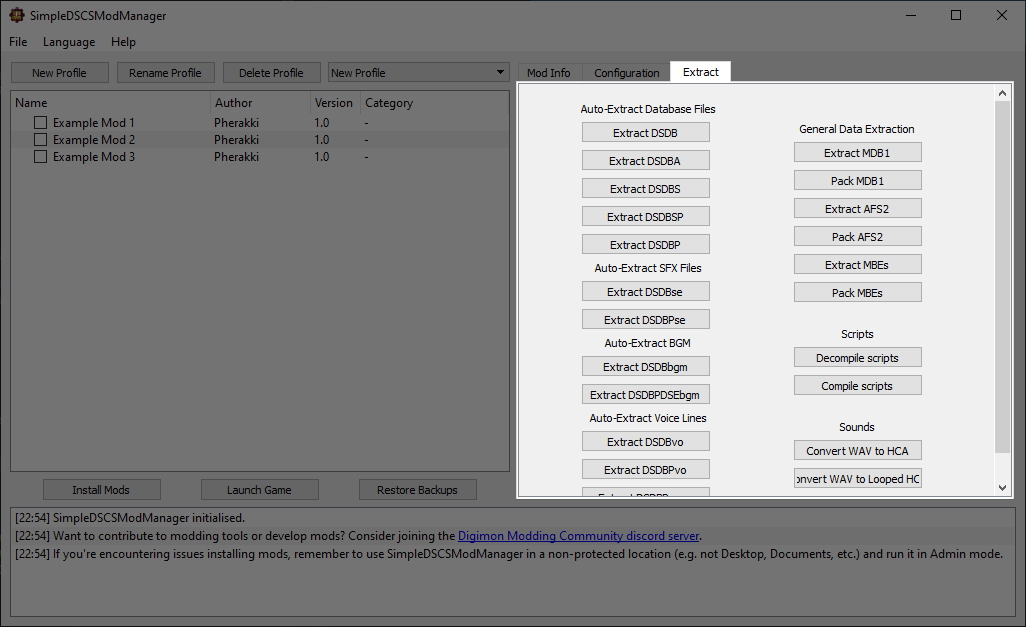
\includegraphics[scale=0.4]{img/modmanager_ui_extracttab.jpg}
\end{center}
\newpage

\section{Game Asset Structure}\label{Section:GameAssets}
\subsection{Asset Archives}
The game data is stored in the \textbf{resources} folder of your game install. The most important files in here are the 12 MVGL archives. One thing to note is that ``MVGL" is not a filetype. There are two kinds of archives in the resource folder: MDB1 and AFS2. MDB1 contains generic compressed data. AFS2 contains HCA sound files.
There are five ``main game data archives", listed here in order of increasing priority:
\begin{itemize}
\item \textbf{DSDB} - MDB1 archive. Contains the majority of the game data.
\item \textbf{DSDBA} - MDB1 archive. Contains overwrite data, mostly censorship data such as the Sistermon Ciel model.
\item \textbf{DSDBS} - MDB1 archive. Contains overwrite data for the PC version with an XBOX Controller.
\item \textbf{DSDBSP} - MDB1 archive. Contains overwrite data for the PC version with a DualShock Controller.
\item \textbf{DSDBP} - MDB1 archive. Contains more overwrite data, mostly data that was provided as DLCs for the Vita and PS4 versions. This is the highest-priority archive that will overwrite all others, and by default the mod manager installs data into this archive.
\end{itemize}
There are two sound effect archives:
\begin{itemize}
\item \textbf{DSDBse} - MDB1 archive. Contains SFX.
\item \textbf{DSDBPse} - MDB1 archive. Contains more SFX.
\end{itemize}
There are two BGM archives:
\begin{itemize}
\item \textbf{DSDBbgm} - AFS2 archive. Contains the game soundtrack.
\item \textbf{DSDBPDSEbgm} - AFS2 archive. Contains (very) small snippets of Digimon anime OST.
\end{itemize}
There are three voice effect archives:
\begin{itemize}
\item \textbf{DSDBvo} - AFS2 archive. Contains the majority of the game's voicelines.
\item \textbf{DSDBPvo} - AFS2 archive. Contains additional voicelines.
\item \textbf{DSDBvous} - AFS2 archives. Contains censorship voicelines.
\end{itemize}
The \textbf{usm} files in the resources folder are video files.

\subsection{Main MDB1 Contents}
An important thing to note before diving into the MDB1 data is that the files inside it follow very strong naming conventions. That is to say, the game will look for assets with very specific filenames for certain game data records. This is both a blessing and a curse; there is in some sense less work to do since the game will automatically pick up and understand what certain files are supposed to be based on their filenames, but that automatic behaviour also means we must adhere to the filename restrictions the game places upon us. This is another reason for the internal complexity of the mod manager. We will cover current knowledge throughout this section.

An MDB1 archive can contain any of the following folders, in addition to model files that are not in any sub-folders:
\begin{itemize}
\item \textbf{data} - Contains the MBE archives that make up the game database, as well as some CSV files that also contribute to the database, in addition to a single image `save\_icon0.png'. The MBE archives are automatically unpacked to folders of CSV files if you tell the mod manager to unpack a specific archive (\textit{i.e.} select an option in the left-hand column of the Extract Tab). The CSV files in the MBE archives have \textbf{UTF-8} encoding. The ``loose" CSV files have \textbf{SHIFT-JIS} encoding. The ``loose" CSV files are:
\begin{itemize}
\item bgm.csv
\item debug\_call\_script.csv
\item debug\_call\_script\_hm.csv
\item se.csv
\item soundtest\_bgm.csv
\item soundtest\_se.csv
\item soundtest\_voice.csv
\item voice.csv
\item voice\_us.csv
\end{itemize}
\item \textbf{message} - Contains MBE archives that store the text for conversations. The MBE archives are automatically unpacked to folders of CSV files if you tell the mod manager to unpack a specific archive (\textit{i.e.} select an option in the left-hand column of the Extract Tab). The CSV files in the MBE archives have UTF-8 encoding.
\item \textbf{text} - Contains MBE archives that store various pieces of text, such as character names and item descriptions. The MBE archives are automatically unpacked to folders of CSV files if you tell the mod manager to unpack a specific archive (\textit{i.e.} select an option in the left-hand column of the Extract Tab). The CSV files in the MBE archives have UTF-8 encoding.
\item \textbf{images} - Contains all image files. For the PC version, these are DDS files with the file extension `img'.
\item \textbf{images\_as} - Contains alternative images that are used when the language is set to Traditional Chinese.
\item \textbf{images\_de} - Contains alternative images that are used when the language is set to German.
\item \textbf{images\_kr} - Contains alternative images that are used when the language is set to Korean.
\item \textbf{script64} - Contains script files that the game attaches to various game contexts, such as battles and maps. The scripts are compiled Squirrel 2.2.4 files. The scripts are automatically decompiled to text files if you tell the mod manager to unpack a specific archive (\textit{i.e.} select an option in the left-hand column of the Extract Tab).
\item \textbf{shaders} - Contains shaders used by the model files. The shaders are plaintext, and written in the Cg language, the language of a deprecated rendering system that is a predecessor-of-sorts to HLSL. The game uses the Cg rendering runtime in conjunction with OpenGL.
\end{itemize}

The files not in any folders are model files, with the exception of a single image file `ui\_title\_logo\_caution.img'. The models can be split into a few categories:
\begin{itemize}
\item \textbf{acc} - Accessory models.
\item \textbf{cam} - Camera models, including those for attacks.
\item \textbf{eff} - Effect files, including those for attacks.
\item \textbf{chr} - Digimon/Enemy models.
\item \textbf{pc} - Player Character models, including outfits.
\item \textbf{npc} - Supporting cast models.
\item \textbf{mob} - Generic NPC models.
\item \textbf{dXXXX} - Dungeon map models, which are split into the same sub-types as the Town map models.
\item \textbf{tXXXX} - Town map models, which are split into the following sub-types:
\begin{itemize}
	\item \textbf{tXXXXf} - The ``Field" model. Contains the mesh that is rendered for the map.
	\item \textbf{tXXXXc} - The ``Collision" model. Contains invisible walls.
	\item \textbf{tXXXXs} - The ``Surface" model. Contains a copy of the floor.
	\item \textbf{tXXXXp} - The ``Position" model. Contains trigger meshes, trigger surfaces, NPC positions, spawn points, etc.
	\item \textbf{tXXXX\_cam} - The ``Camera" model. Contains the camera for the map.
	\item \textbf{tXXXX\_hide} - The ``Hide" model. These are meshes that can become transparent when the player enters a certain trigger, usually to prevent the mesh from obscuring the camera. Linked to trigger surfaces in the ``Position" model.
\end{itemize}
\item \textbf{ui} - Various bits of the user interface, which are all implemented as 3D models.
\end{itemize}
In addition to these, there are a number of other models that aren't fully categorised.

The models themselves are split between nine filetypes:
\begin{itemize}
\item \textbf{name} - [Required] Contains bone names and material names.
\item \textbf{skel} - [Required] Contains the ``rest pose" of the model, which is equivalent to the first frame of the ``base animation" for that model. A few models have different skels and first-frame-of-base-animations, but this is suspected to be a mistake on the part of the developer, and the game corrects for this regardless.
\item \textbf{geom} - [Required] Contains the ``bind pose" of the model, the materials, texture names, lights, and cameras.
\item \textbf{anim} - [Required] Contains animation data. 
\item \textbf{detr} - [Optional] Unknown, seems to contain walk paths for NPCs in maps.
\item \textbf{phys} - [Optional] Contains colliders for maps.
\item \textbf{note} - [Optional] Unknown, seems to affect the rendering of text.
\item \textbf{sprk} - [Optional] Unknown, seems to contain particle effects.
\item \textbf{navi} - [Optional] Unknown, used in ``autoran" models. May be another kind of walk path.
\end{itemize}

All files with the same filename are associated with the same model --- \textit{e.g.} `t0101.name` and `t0101.skel` would be parts of the same model. An exception is made for the Anim files - the file `t0101.anim` would be interpreted as the ``base animation" for the model `t0101' if the other files for that model also exist. This is an animation that is constantly playing, and for many models it contains no data. There are also some ``overlay animations" for models. These are identified by suffixes being attached to the filename, \textit{e.g.} for a model with a base animation called `chr003.anim`, there might be an overlay animation called `chr003\_ba01.anim`. Many of these overlay animations have strict naming conventions, such that the game can automatically know where an animation file for a certain action should exist. Other suffixes are arbitrary. A few of the suffixes are:
\begin{itemize}
\item \textbf{ba01} - Battle Attack 1. The animation attached to the `basic attack' function in battles.
\item \textbf{ba02} - Battle Attack 2. The animation attached to the `skill' function in battles.
\item \textbf{bb01} - Battle Backwards 1. An animation for moving backwards.
\item \textbf{bd01} - Battle Damage 1. The animation played when receiving damage.
\item \textbf{bd02} - Battle Damage 2. The animation played when being knocked down.
\item \textbf{bd03} - Battle Damage 3. The animation played when getting back up again.
\item \textbf{bg01} - Battle Guard 1. The animation played when received damage while guarding.
\item \textbf{bn01} - Battle Normal 1. The ``rest" animation played during battles.
\item \textbf{br01} - Battle Run 1. The ``run" animation played in battles.
\item \textbf{bs01} - Battle Special 1. The animation for the ``Special Skill 1'.
\item \textbf{bs02} - Battle Special 2. The animation for the ``Special Skill 2'.
\item \textbf{bv01} - Battle Victory 1. The animation played when a battle if won.
\item \textbf{fe01} - Field Eat 1. The animation played when eating food in the DigiFarm.
\item \textbf{fn01} - Field Normal 1. The animation played when ``resting" in the field.
\item \textbf{fr01} - Field Run 1. The ``run" animation played in the field.
\item \textbf{fw01} - Field Walk 1. The ``walk" animation played in the field.
\item \textbf{fw02} - Field Walk 2. A slower ``walk" animation played in the field.
\end{itemize}
The game will fall back to alternatives if animations do not exist in some cases, for example the game will use `br01' instead of `fr01' if `fr01' does not exist. For this reason, many \textbf{chr} models do not have most of the `field' animations defined.

Other overlay animations seem to have names that are not strictly enforced by the game, but the developers still use a naming convention for.
\begin{itemize}
\item \textbf{e} - ``Emote" animations used in conversations.
\item \textbf{ev} - ``Event" animations used for in-engine cutscenes, usually suffixed with a chapter and number.
\item \textbf{fXX\_mXX} - Face and Mouth animations. These change the facial expression.
\end{itemize}

\subsection{SFX MDB1 Contents}
The SFX MDB1 archives just contain a folder called ``sound", which contains HCA files (although they may have the file extension `snds'). 

\subsection{BGM AFS2 Contents}
The BGM AFS2 archives are standard AFS2 archives. The contents are extracted with filenames corresponding to their entry number in the AFS2, in \textbf{hexadecimal} (not decimal). The game finds these files using \textbf{bgm.csv}, which is in the \textbf{DSDB} archive. This csv gives each member of a AFS2 archive a name for internal use within the game.  The `\textbf{cri\_contents\_id}' column gives the file index, in \textbf{decimal}. For example, an entry in the csv with a cri\_contents\_id of \textbf{17} would correspond to the file \textbf{000011.hca}.

Note also that the name of the AFS2 archive the file belongs to is given. The game will dynamically load data from whatever name you put here for an AFS2. So, you can add new BGM tracks by creating a new AFS2 file and referring to the name of the AFS2 file in that column.

\subsection{VFX AFS2 Contents}
The VFX AFS2 archives are standard AFS2 archives. The contents are handled identically to the BGM files, except that the csv that assigns each track a name used by the game is \textbf{voice.csv} and \textbf{voice\_us.csv}.
\newpage

\section{Creating SDMM Mods}
\subsection{Basic Mod Structure}
Mods require two things at a minimum:
\begin{itemize}
\item A folder called \textbf{modfiles}
\item A file called \textbf{METADATA.json} containing a JSON dictionary
\end{itemize}
The "modfiles" folder contains the mod data. \textbf{For now, we will just describe how to add data that goes in the `Main Asset Data' archives}, \textit{i.e.} data that will be inserted into \textbf{DSDBP}. We will describe how to add data that should go into other archives and loose files, in section \ref{Section:InstallingNonMainData}. It should be structured like an unpacked game archive, with the "modfiles" folder in the place of the folder the unpacked game data would be in (i.e. "modfiles" might contain the folders "data/", "message/", "script64/" \textit{etc}).\\
\begin{center}
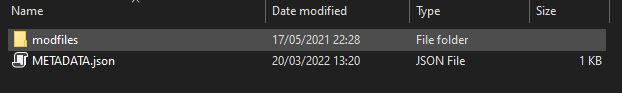
\includegraphics[scale=0.6]{img/mod_contents.jpg}
\end{center}
The \textbf{METADATA.json} can contain five main keys:
\begin{itemize}
\item Name
\item Author
\item Version
\item Category
\item Description
\end{itemize}
All of these should be strings (\textit{i.e.} inside quotes), and additionally the "Description" field may be written in HTML. 
\begin{lstlisting}[language=json,firstnumber=1]
{
    "Name": "Example Mod 1",
    "Author": "Pherakki",
    "Version": "1.0",
    "Category": "Utilities",
    "Description": "Short Description"
}
\end{lstlisting}
\noindent The ``Description" entry field is very restrictive since the description must be all on a single line; if you want to have a more complex description making use of more HTML features, you can also add a `\textbf{DESCRIPTION.html}' file to your mod that will take priority over the Description member of the metadata file.
\begin{center}
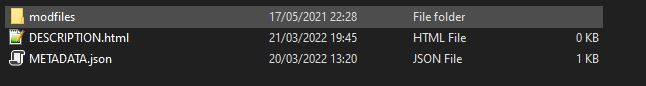
\includegraphics[scale=0.6]{img/mod_contents_html.jpg}
\end{center}

\newpage
\subsection{Adding and Editing Files}
The mod manager gives you several tools to edit the game data. The mod manager uses two core ideas to patch the game: \textbf{filetypes} and \textbf{rules}. The mod manager will scan your mod, and automatically identify certain files (such as csv files) as being specific filetypes. The mod manager will then use that file, in conjunction with a \textbf{rule}, to merge those files into the game data. Every filetype known to the mod manager has a default rule, meaning that you can just put a bunch of files into a mod and the mod manager will patch them into the game using the most commonly-desired method. You can change precisely how the mod manager will use your filetype by specifying different \textbf{rule}s, but we will see how to do this in section \ref{Section:BuildScripts}. For now, let's take a look at the various filetypes the mod manager will automatically recognise and patch into the game data. Note that, if a file is not recognised as any of these filetypes, the mod manager will copy the file into the game data ``normally" which will cause it to take priority over a vanilla file with the same name, if one exists. In each of these sections, we will list the default rule that each filetype uses so we can refer back to these later.

This can get a bit complicated and difficult to describe in words. It's a good idea to download a few mods designed for SDMM, and cross-reference how they are set up and what data they contain with the descriptions given in this section. Remember also that this document is a reference guide! There are a huge number of possible things to mod in this game, and so instructions on how to mod a specific piece of the game are not included in this guide, lest it grow to an unmaintainable size and need extremely frequent updates. You can refer to separate articles on how to implement specific bits of functionality, which should be kept in the Documentation folder of the SDMM GitHub repository.

\subsubsection{CSV Files}
\textbf{File Types}
\begin{itemize}
\item \textbf{.csv Extension}\\
To edit CSV files, add a csv file with the same path as the csv you want to edit. For example, if you want to edit \textbf{data/bgm.csv}, add a file called \textbf{bgm.csv} to a folder called \textbf{data} inside the \textbf{modfiles} directory of your mod. The first line of your mod CSV is ignored, so you can put the header of the original file in there to help keep track of what the columns are. In the following rows (which I will refer to as \textbf{records}), you can enter the data you wish to add to the game. Typically, the very first cell of the record is an `ID' column. In some rare cases, the `ID' is two or more cells. If the `ID' of a record in your modded CSV is the same as one that already exists, your game data will be used to edit the vanilla game data. If it's a new ID, then it will make a new record.\\\\
\underline{\textit{Default Rule: mberecord\_merge}}\\
The default behaviour is to replace (or add) the entire record corresponding to the ID specified in your file with the data contained in that row. If you leave a cell in the csv blank, the cell will act as if it is ``transparent" and will not overwrite the original value that was in that cell with your data. You can use this to make surgical edits, such as editing a single value inside a record.
\end{itemize}
\textbf{Rules}
\begin{itemize}
	\item \textbf{mberecord\_merge}\\
	Replace (or add) the entire record corresponding to the ID specified in your file with the data contained in that row. If you leave a cell in the csv blank, the cell will act as if it is ``transparent" and will not overwrite the original value that was in that cell with your data.
	\item \textbf{mberecord\_overwrite}\\
	Replace (or add) the entire record corresponding to the ID specified in your file with the data contained in that row. This completely overwrites the entire record.
	\item \textbf{mberecord\_append}\\
	Strips the padding data from the current record data, appends the data in your records on the end, and re-pads with the padding characters. Default padding character is \textbf{0}. This can be changed by giving a padding character as a rule argument in a build script, \textit{e.g.} [filepath, ``mberecord\_append", ``-1"].
	\item \textbf{mberecord\_remove}\\
	Strips the padding data from the current record data, removes any entries in your records from the current record data, and re-pads with the padding characters. Default padding character is \textbf{0}. This can be changed by giving a padding character as a rule argument in a build script, \textit{e.g.} [filepath, ``mberecord\_remove", ``-1"].
\end{itemize}
\subsubsection{MBE Tables}
\textbf{File Types}
\begin{itemize}
\item \textbf{.csv Extension}\\
MBE tables are handled very similarly to .csv files, since the MBE data is unpacked to .csv files by DSCSTools (which the mod manager uses to unpack and re-pack the game data). The difference between MBE tables and csv files is that the mod manager will \textbf{recognise a file contained inside a folder ending with `.mbe'} as part of an MBE table. For example, \textbf{data/charname.mbe/Sheet.csv} will be recognised as an MBE table, whereas  \textbf{data/charname/Sheet.csv} will be recognised as a csv file.

Similarly to csv files, you need only include the data you wish to edit or add inside your MBE tables. An additional consideration in this case is that MBEs often contain multiple tables --- they unpack to several csv files. You only need to include the files that you edit with your mod. The mod manager will take care of merging this in to the MBE alongside the other tables. Other than this, editing MBE tables is identical to editing csv files.\\\\
\underline{\textit{Default rule: mberecord\_merge}}
\end{itemize}
\textbf{Rules}\\
Rules are identical to the CSV rules.

\subsubsection{Script Files}
\textbf{File Types}
\begin{itemize}
\item \textbf{.txt Extension}\\
Script files are identified as files with a \textbf{.txt} extension inside the \textbf{script64} folder. \textbf{Files outside of script64 will not be recognised as script files}. Any text inside your script file will be appended to the existing scripts. Due to the dynamic nature of the Squirrel programming language, if you create a function with the same name as a function that already exists, your function will overwrite that function.\\\\
\underline{\textit{Default rule: squirrel\_concat}}

\item \textbf{.sqmod Extension}\\
Sometimes, you don't want to add or overwrite entire functions, but rather you want to extend pre-existing functions or replace function calls. To do this, you can use a `.sqmod' file. This is a JSON file containing a list of dictionaries, each of which implements a Squirrel Mod rule. A list of these rules is given below. This list of rules will grow as the mod manager is updated.
\begin{itemize}
\item This rule adds code immediately before the first function definition in the script file.
\begin{itemize}
\item \textbf{add\_preamble}: A list of strings. Each string is a line of code to add to the function.
\end{itemize}

\item This rule will add the code specified in the `with' argument to the function assign to `extend\_func'.
\begin{itemize}
\item \textbf{extend\_func} : Assigned the name of the function you want to add code to.
\item with : A list of strings. Each string is a line of code to add to the function.
\end{itemize}

\item This rule performs a straight find-and-replace of the text given to `replace' with the text given to `with'. \textbf{Can lead to very unexpected results if not used carefully}.
\begin{itemize}
\item \textbf{replace}: The string to replace.
\item \textbf{with}: The string to fill in the replacements with.
\end{itemize}

\item This rule will find the function call specified to `replace\_call' and replace it with the function call given to `with'. Function arguments are identified by curly braces containing a hash alongside an argument ID number. These arguments can be re-used in the `with' statement to re-arrange or adjust function arguments.
\begin{itemize}
\item \textbf{replace\_call}: Receives the function call to replace (see the example given at the bottom of the sqmod documentation)
\item with: Receives the edited function call.
\end{itemize}

\item This rule functions identically to `replace\_call', but only works inside the functions named inside the `funcs' argument.
\begin{itemize}
\item \textbf{replace\_call\_in\_funcs}: Receives the function call to replace (see the example given at the bottom of the sqmod documentation)
\item with: Receives the edited function call.
\item funcs: A list of strings. Each string is the name of a function that this find-and-replace will apply to.
\end{itemize}
\end{itemize}
\end{itemize}

\textit{Example sqmod file from the skip dialogue mod. globalSkipTextMode and globalSkipAnimMultiplier are variables added with a .txt script file.}
\begin{lstlisting}[language=json,firstnumber=1]
[
    {
        "replace_call": "this.Talk.PlayAnimation({#0}, {#1}, {#2}, {#3})",
        "with": "this.Talk.PlayAnimation({#0}, {#1}, globalSkipTextMode ? ({#2}/globalSkipAnimMultiplier) : ({#2}), {#3})"
    },
    {
        "replace_call": "this.Vista.PlayAnimation({#0}, {#1}, {#2}, {#3})",
        "with": "this.Vista.PlayAnimation({#0}, {#1}, globalSkipTextMode ? ({#2}/globalSkipAnimMultiplier) : ({#2}), {#3})"
    }
]
\end{lstlisting}

\underline{\textit{Default rule: squirrel\_modify}}\\

\textbf{Rules}
\begin{itemize}
	\item \textbf{squirrel\_concat}\\
	Appends the text in a file onto the end of the current source code.
	\item \textbf{squirrel\_modify}\\
	Parses the file as a ``sqmod" file, and applies those edits to the current source code following the sqmod scheme.
\end{itemize}
\subsubsection{Model Files}
\textbf{File Types}
\begin{itemize}
\item \textbf{.name Extension}\\
A plain `name' file. Overwrites the pre-existing file by default.\\\\
\underline{\textit{Default rule: overwrite}}
\item \textbf{.skel Extension}\\
A plain `skel' file. Overwrites the pre-existing file by default.\\\\
\underline{\textit{Default rule: overwrite}}
\item \textbf{.geom Extension}\\
A plain `name' geom. Overwrites the pre-existing file by default.\\\\
\underline{\textit{Default rule: overwrite}}
\item \textbf{.anim Extension}\\
A plain `anim' file. Overwrites the pre-existing file by default.\\\\
\underline{\textit{Default rule: overwrite}}
\item \textbf{.mdledit Extension}\\
A `.mdledit' file allows you to make specific edits to model files. Currently, it is an extremely limited proof-of-concept that allows you to add new NPCs to maps only.

The mdledit file is a JSON file consisting of a dictionary of mdledit rules. The dictionary can have repeated entries. Each rule is itself given a dictionary of parameters. A list of mdledit rules and their parameters are given below.
\begin{itemize}
\item \textbf{editNPC}.
\begin{itemize}
\item \textit{id} - [Required]\\The NPC ID.
\item \textit{position} - [Optional, Default: [0, 0, 0]]\\A list of 3 elements containing the [x, y, z] coordinates of the NPC in the map.
\item \textit{rotation} - [Optional, Default: [1, 0, 0, 0]] \\A list of 4 elements containing a quaternion rotation, in WXYZ ordering, for the NPC.
\item \textit{scale} - [Optional, Default: [1, 1, 1]] \\A list of 3 elements containing the [x, y, z] scales for the NPC.
\end{itemize}
\end{itemize}
\end{itemize}

\underline{\textit{Default rule: mdledit\_name/skel/geom/anim}}\\\\
\textbf{Rules}
\begin{itemize}
\item \textbf{mdledit\_name}\\
Applies the mdledit editing scheme to name files.
\item \textbf{mdledit\_skel}\\
Applies the mdledit editing scheme to skel files.
\item \textbf{mdledit\_geom}\\
Applies the mdledit editing scheme to geom files.
\item \textbf{mdledit\_anim}\\
Applies the mdledit editing scheme to anim files.
\end{itemize}

\subsubsection{Including and Overwriting Vanilla Files}
\begin{itemize}
\item \textbf{.request Extension}\\
Sometimes, you may need to re-use a vanilla file inside your mod. If this is the case, you don't need to distribute this asset with your mod --- just include a Request file in the location where you want that file to be. For example, if you want to include the file `chr003.name', add the file `chr003.name.request' to your mod as a blank text file. If you request the version of that file from a specific archive, put the name of that archive inside the Request file (\textit{e.g.} if you want to include the version of `chr783.name' from DSDB, write the letters `DSDB' in the Request file).

\underline{\textit{Default rule: request\_file}}
\item \textbf{Any other file}
Any other file just gets given the ``overwrite" rule, which copies the file over the vanilla file.\\
\underline{\textit{Default rule: overwrite}}
\end{itemize}
\textbf{Rules}
\begin{itemize}
	\item \textbf{request\_file}\\
	Implements the `request' system.
	\item \textbf{overwrite}\\
	Copies the file over the vanilla file.
\end{itemize}


\newpage
\subsection{Installing Data Outside of DSDBP}\label{Section:InstallingNonMainData}
The vast majority of mods will want to install data into the DSDBP archive. For this, and backwards-compatibility reasons, the mod manager will install all data into DSDBP. However, some data, such as SFX and music, should go into their own archives. We can tell the mod manager to switch to a mode where it can install data to several locations by adding the line \textbf{"FormatVersion": 2} to the \textbf{METADATA.json}.
\begin{lstlisting}[language=json,firstnumber=1]
{
    "FormatVersion": 2,
    "Name": "Example Mod 1",
    "Author": "Pherakki",
    "Version": "1.0",
    "Category": "Utilities",
    "Description": "Short Description"
}
\end{lstlisting}
You can then install data to specific archives by \textbf{making a folder with the name of the archive} inside the \textbf{modfiles} folder, and putting all data to go into that archive inside that folder. For example, to recover the previous behaviour of putting all data into DSDBP, create a folder called \textbf{DSDBP} inside your \textbf{modfiles} folder and put all data inside it. The mod manager will automatically recognise the names of archives, and if a folder is not recognised as one, its contents will be installed as a folder rather than inside an archive.

\textbf{You are recommended to keep all `main game data archive' data inside DSDBP.} For adding new AFS2 data, you may find it easiest to use the dynamic-archive-loading features of DSCS by packing your HCA data into the AFS2 archives with the mod manager yourself, including the entire AFS2 archive inside the \textbf{modfiles} folder, and referring to the archive inside the appropriate csv loader file (\textit{e.g.} bgm.csv). Remember, \textbf{DSDBP is an overwrite archive}, so putting your edits to \textit{e.g.} bgm.csv inside \textbf{DSDBP} will work fine since the mod manager will patch them into the game data appropriately for you. 

You are highly discouraged from inserting new data into the \textbf{DSDB} archive. This is a very large archive that will take some time to re-build, as well as not having much spare room in the first place. You are best off sticking to DSDBP. Note that data packed into MDB1 archives will be compressed, and can actually hold many times more data than the 4 GiB limit would suggest. In general, you should only need to use the \textbf{"FormatVersion": 2} option if you're looking to install audio data or loose files. Specific articles that go into detail for adding data with new AFS2 archives should exist in the mod manager documentation if you want an in-depth example.

\subsection{Readying your Mod for Distribution}
The mod manager expects mods to either be contained inside \textbf{zip} files, or in a folder containing the \textbf{modfiles} and \textbf{METADATA.json} files. For distribution, you should pack your mod into a \textbf{zip} file. The mod manager will recognise zip files in two formats:
\begin{itemize}
\item The zip file contains the \textbf{modfiles}, \textbf{METADATA.json} \textit{etc.} in the top level of the zip archive, \textit{i.e.} unpacking the zip creates \textbf{modfiles}, \textbf{METADATA.json} in the same location as the zip file.
\item The zip file contains a single folder, which itself contains the \textbf{modfiles}, \textbf{METADATA.json} \textit{etc.} This folder must have the same name as the zip file itself. For example, you could have a zip file called \textbf{MyMod.zip} that contains a folder called \textbf{MyMod}, which itself contains the contents of your mod.
\end{itemize}

\newpage
\section{SDMM Mod-Building Features}
\subsection{Softcodes}
\subsubsection{The Need for Softcodes}
You may have noticed that the IDs for records in the game database are hardcoded. These IDs appear in the MBE files, in model files, in script files, and even in filenames. For example, the file `chr003.name' Uses the digimon ID `3' in the filename. This ID is hard-linked to various MBE records in the game by the game logic.

In some ways, this is good, since we have less work to do. However, since IDs have to be hardcoded in this way, what happens when two mods both want to add something new under a new ID, and accidently use the same ID? The two mods will conflict, and one will gain precedence over the other. This is not a good situation for the modular addition of data to the game, since two mods can very easily become incompatible in this way.

This critical issue is behind the introduction of \textbf{Softcodes}. Softcodes are tags that the mod manager can detect, and automatically fill in with a mod-manager-given ID. Several games designed for mods do similar things out-of-the-box, and give IDs to new records when mods are loaded by the game. Unfortunately, since DSCS is \textit{not} designed for mods, we have to create a similar system ourselves.

The basic Softcode syntax is
\begin{center}\textbf{[Category::Key]}
\end{center}
where `Category' is a particular collection of IDs, and `Key' is that name of an ID in that collection. A list of all Categories is given in section \ref{Section:SoftcodeList}.

Some softcodes have sub-categories. You can access sub-categories using a \textbf{|} character. Softcodes can have arbitrarily deep numbers of sub-categories, although in practice this does not ever exceed three.

This still only returns a single number. An example of a sub-category would be an enemy variant of a Digimon. The number you would get is the ID of the variant.
\begin{center}
\textbf{[Category::Key|SubCategory::Key2|SubSubCategory::Key3]}
\end{center}

Some IDs are expected by the game to be in certain formats. Many softcodes define functions to assist with this --- for example, padding a code to always be 3 digits in size. These functions are also given per category in \ref{Section:SoftcodeList}. You can only call a function on the \textbf{final key of a softcode}, because this is the number that the softcode resolves to.

The function is called by adding an extra `::' after the key, followed by the name of the function, followed by an open parenthesis and a closed parenthesis.
\begin{center}
\textbf{[Category::Key|SubCategory::Key2|SubSubCategory::Key3::function()]}
\end{center}

The most important function of softcodes is the ability to add new IDs using them. In order to use a softcode, simply write a softcode with a key attached to a category in one of your files, for example \textbf{[Item::MyNewItem]}. If the key \textbf{MyNewItem} does not exist, the mod manager will automatically assign it a new ID from the \textbf{Item} category. A nice feature of this system is that other mods will also be able to refer to these keys, and build on or edit other mods in this way.

As previously mentioned, some softcodes need to be used in the names of files. This will be covered in section \ref{Section:BuildScripts}.

\textbf{Please note that a complete set of required softcodes is not included with v\cymisversion~of SDMM}. This version released with a number of softcodes that should be sufficient for the most common modding needs. Additional softcodes will be added over time, eventually covering the entire database. You can always hardcode other IDs for now, with the option of updating these to softcodes when the appropriate codes are ready.

\subsubsection{Softcode Aliases}
Softcodes can sometimes get very long. To aid with this, you can \textbf{alias} chunks of softcodes in order to make them shorter or more idiomatic. For example, instead of writing
\begin{center}
	[Dungeon\_CS::d90|SubArea::d9002|NPC::npc\_0008]
\end{center}
you might prefer to write
\begin{center}
	[ShibuyaNPCs::npc\_0008]
\end{center}
You can do this by adding an \textbf{ALIASES.json} to you mod in the same place as the \textbf{METADATA.json}. The \textbf{ALIASES.json} is a JSON dict containing string : string pairs. The left string is the alias, and the right string is the original piece of the softcode you want to replace. Note that Aliases are expected to \textbf{end with a category}. For example, the Alias given above would be defined in a file as
\begin{lstlisting}[language=json,firstnumber=1]
{
    "ShibuyaNPCs" : "Dungeon_CS::d90|SubArea::d9002|NPC"
}
\end{lstlisting}

\noindent You can equivalently define it as
\begin{lstlisting}[language=json,firstnumber=1]
{
    "ShibuyaNPCs::" : "Dungeon_CS::d90|SubArea::d9002|NPC::"
}
\end{lstlisting}

\noindent if you prefer, since the mod manager will automatically pad the right-hand side of the aliases up to two `:' characters. This is so that the softcodes you write in your files will always be in the softcode format, \textit{i.e.} \textbf{[Category::Key]}, \textbf{[Category::Key|SubCategory::Key2]}, \textbf{[Category::Key::function()]} \textit{etc.}, so that the mod manager can easily find them. This restriction may be lifted in the future so that individual key values can be aliased, but it is not a priority.

Note that aliases are specific to \textit{your mod only}, so they are merely a convenience for you alone. Other mods are not able to access the aliases you define, and you are not able to access the aliases of other mods.

\newpage
\subsubsection{Softcode List}\label{Section:SoftcodeList}
\begin{itemize}
	\item \textbf{BattleBGM}
	\begin{itemize}
		\item Purpose: IDs for Battle BGM tracks.
		\item Value: Return the ID without modifications.
		\item Methods: None
		\item Children: None
	\end{itemize}
	
	\item \textbf{Digimon}
	\begin{itemize}
		\item Purpose: IDs for Digimon and Battle Entities.
		\item Value: Return the ID without modifications.
		\item Methods:
		\begin{itemize}
			\item 3ID : Pad ID to the left with 0s to a width of 3 characters.\\
			\textit{e.g.} $1 \rightarrow 001$
			\item 4ID : Pad ID to the left with 0s to a width of 3 characters, and add an extra 1 to the left.\\
			\textit{e.g.} $1 \rightarrow 1001$
			\item filename : Pad ID to the left with 0s to a width of 3 characters and add `chr' to the left.\\
			\textit{e.g.} $1 \rightarrow$ chr001
		\end{itemize}
		\item Children:
		\begin{itemize}
			\item \textbf{Digimon}$\rightarrow$\textbf{EnemyVariant}
		\end{itemize}
	\end{itemize}
	
	\item \textbf{Digimon}$\rightarrow$\textbf{EnemyVariant}
	\begin{itemize}
		\item Purpose: IDs for different statlines for enemy Battle Entities.
		\item Value: Return the ID without modifications.
		\item Methods: None
		\item Children: None
	\end{itemize}
	
	\item \textbf{Dungeon\_CS}
	\begin{itemize}
		\item Purpose: IDs Dungeon-type Areas.
		\item Value: Pad ID to the left with 0s to a width of 2 characters, add d to the front of the ID.\\
		\textit{e.g.} 1$\rightarrow$d01\\
		\textit{e.g.} 101$\rightarrow$d101
		\item Methods:
		\begin{itemize}
			\item ID : Pad ID to the left with 0s to a width of 2 characters.\\
			\textit{e.g.} 1$\rightarrow$01\\
			\textit{e.g.} 101$\rightarrow$101
		\end{itemize}
		\item Children:
		\begin{itemize}
			\item \textbf{Dungeon\_CS}$\rightarrow$\textbf{SubArea}
		\end{itemize}
	\end{itemize}
	
	\item \textbf{Dungeon\_CS}$\rightarrow$\textbf{SubArea}
	\begin{itemize}
		\item Purpose: IDs for SubAreas of Dungeon-type Areas.
		\item Value: Pad ID to the left with 0s to a width of 2 characters, add the parent value to the front of the ID.\\
		\textit{e.g.} 1$\rightarrow$ d0101\\
		\textit{e.g.} 1$\rightarrow$ d10101
		\item Methods:
		\begin{itemize}
			\item ID:  Pad ID to the left with 0s to a width of 2 characters.\\
			\textit{e.g.} 1$\rightarrow$ 01
			\item MapID:  Pad ID to the left with 0s to a width of 2 characters, add the parent ID to the front of the ID.\\
			\textit{e.g.} 1$\rightarrow$ 101\\
			\textit{e.g.} 1$\rightarrow$ 10101
			\item battleFile: SubArea Value with `b' on the end of the file.\\
			\textit{e.g.} 1$\rightarrow$ d0101b\\
			\textit{e.g.} 1$\rightarrow$ d10101b
			\item collisionFile: SubArea Value with `c' on the end of the file.\\
			\textit{e.g.} 1$\rightarrow$ d0101c\\
			\textit{e.g.} 1$\rightarrow$ d10101c
			\item positionFile: SubArea Value with `p' on the end of the file.\\
			\textit{e.g.} 1$\rightarrow$ d0101p\\
			\textit{e.g.} 1$\rightarrow$ d10101p
			\item surfaceFile: SubArea Value with `s' on the end of the file.\\
			\textit{e.g.} 1$\rightarrow$ d0101s\\
			\textit{e.g.} 1$\rightarrow$ d10101s
			\item fieldFile: SubArea Value with `f' on the end of the file.\\
			\textit{e.g.} 1$\rightarrow$ d0101f\\
			\textit{e.g.} 1$\rightarrow$ d10101f
			\item cameraFile: SubArea Value with `\_cam' on the end of the file.\\
			\textit{e.g.} 1$\rightarrow$ d0101\_cam\\
			\textit{e.g.} 1$\rightarrow$ d10101\_cam
			\item hideablesFile: SubArea Value with `\_hide' on the end of the file.\\
			\textit{e.g.} 1$\rightarrow$ d0101\_hide\\
			\textit{e.g.} 1$\rightarrow$ d10101\_hide
		\end{itemize}
		\item Children:
		\begin{itemize}
			\item \textbf{Dungeon\_CS}$\rightarrow$\textbf{SubArea}$\rightarrow$\textbf{NPC}
		\end{itemize}
	\end{itemize}
	
	\item \textbf{Dungeon\_CS}$\rightarrow$\textbf{SubArea}$\rightarrow$\textbf{NPC}
	\begin{itemize}
		\item Purpose: IDs for NPCs in the SubAreas of Dungeon-type Areas.
		\item Value: Returns the ID without modifications.
		\item Methods:
		\begin{itemize}
			\item bone\_name: Pads the ID to the left with 0s to a width of 4 characters, and add `npc\_' to the left.\\
			\textit{e.g.} 1$\rightarrow$npc\_0001
		\end{itemize}
		\item Children: None
	\end{itemize}
	
	\item \textbf{Dungeon\_HM}
	\begin{itemize}
		\item Identical definition to \textbf{Dungeon\_CS}.
	\end{itemize}
	
	\item \textbf{Dungeon\_HM}$\rightarrow$\textbf{SubArea}
	\begin{itemize}
		\item Identical definition to \textbf{Dungeon\_CS}$\rightarrow$\textbf{SubArea}.
	\end{itemize}
	
	\item \textbf{Dungeon\_HM}$\rightarrow$\textbf{SubArea}$\rightarrow$\textbf{NPC}
	\begin{itemize}
		\item Identical definition to \textbf{Dungeon\_CS}$\rightarrow$\textbf{SubArea}$\rightarrow$\textbf{NPC}.
	\end{itemize}
	
	\item \textbf{Field\_CS}
	\begin{itemize}
		\item Purpose: IDs for all Areas used in the master list of Areas for Cyber Sleuth.
		\item Value: Returns the ID without modifications.
		\item Methods: None
		\item Children: None
	\end{itemize}
	
	\item \textbf{Field\_HM}
	\begin{itemize}
		\item Purpose: IDs for all Areas used in the master list of Areas for Hacker's Memory.
		\item Value: Returns the ID without modifications.
		\item Methods: None
		\item Children: None
	\end{itemize}
	
	\item \textbf{Item}
	\begin{itemize}
		\item Purpose: IDs for Items.
		\item Value: Returns the ID without modifications.
		\item Methods: None
		\item Children: None
	\end{itemize}
	
	\item \textbf{Shop}
	\begin{itemize}
		\item Purpose: IDs for Shops.
		\item Value: Returns the ID without modifications.
		\item Methods: None
		\item Children: None
	\end{itemize}
	
	\item \textbf{ShopLimitLineup}
	\begin{itemize}
		\item Purpose: IDs for LimitLineup entries for shops.
		\item Value: Returns the ID without modifications.
		\item Methods: None
		\item Children: None
	\end{itemize}
	
	\item \textbf{ShopLineup}
	\begin{itemize}
		\item Purpose: IDs for Shop inventories.
		\item Value: Returns the ID without modifications.
		\item Methods: None
		\item Children: None
	\end{itemize}
	
	\item \textbf{ShopText}
	\begin{itemize}
		\item Purpose: IDs for text displayed in shops.
		\item Value: Returns the ID without modifications.
		\item Methods: None
		\item Children: None
	\end{itemize}
	
	\item \textbf{Skill}
	\begin{itemize}
		\item Purpose: IDs for Battle Skills.
		\item Value: Returns the ID without modifications.
		\item Methods: None
		\item Children: None
	\end{itemize}
	
	\item \textbf{Speakers}
	\begin{itemize}
		\item Purpose: IDs for new Speakers in dialogues.
		\item Value: Returns the ID without modifications.
		\item Methods: None
		\item Children: None
	\end{itemize}
	
	\item \textbf{SupportSkill}
	\begin{itemize}
		\item Purpose: IDs for Battle Support Skills.
		\item Value: Returns the ID without modifications.
		\item Methods: None
		\item Children: None
	\end{itemize}
	
	
	\item \textbf{Town\_CS}
	\begin{itemize}
		\item Identical definition to \textbf{Dungeon\_CS}, except with the $d$ padding character replaced with $t$.
	\end{itemize}
	\item \textbf{Town\_CS}$\rightarrow$\textbf{SubArea}
	\begin{itemize}
		\item Identical definition to \textbf{Dungeon\_CS}$\rightarrow$\textbf{SubArea}, except with the $d$ padding character replaced with $t$.
	\end{itemize}
	\item \textbf{Town\_CS}$\rightarrow$\textbf{SubArea}$\rightarrow$\textbf{NPC}
	\begin{itemize}
		\item Identical definition to \textbf{Dungeon\_CS}$\rightarrow$\textbf{SubArea}$\rightarrow$\textbf{NPC}.
	\end{itemize}
	\item \textbf{Town\_HM}
	\begin{itemize}
		\item Identical definition to \textbf{Dungeon\_CS}, except with the $d$ padding character replaced with $t$.
	\end{itemize}
	\item \textbf{Town\_HM}$\rightarrow$\textbf{SubArea}
	\begin{itemize}
		\item Identical definition to \textbf{Dungeon\_CS}$\rightarrow$\textbf{SubArea}, except with the $d$ padding character replaced with $t$.
	\end{itemize}
	\item \textbf{Town\_HM}$\rightarrow$\textbf{SubArea}$\rightarrow$\textbf{NPC}
	\begin{itemize}
		\item Identical definition to \textbf{Dungeon\_CS}$\rightarrow$\textbf{SubArea}$\rightarrow$\textbf{NPC}.
	\end{itemize}
	
\end{itemize}
\newpage
\subsection{Mod Manager Variables}
\subsubsection{What are Mod Manager Variables?}
The mod manager can keep track of certain variables that mods can share. The mod manager doesn't contain any by default, but mods can easily define and set new variables. For example, a shop could be set up to sell a certain type of item only. This list of items could be appended to by other mods, allowing the inventory of this shop to change depending on what mods are installed.

Mod manager variables share the same syntax as softcodes.

To use Mod Manager Variables, create a file called \textbf{Variables.txt} in the same location as your \textbf{METADATA.json}. Define a new variable by writing the name of the list in the text file. On each new line, you can then edit the variable using an \textit{operator}. The details how to edit these variables are given in section \label{Section:VariableTypesList}. Note that \textbf{you can use softcodes inside the Variables.txt!}

As an example, let's say we've defined a new \textbf{VarList} called \textbf{MyListOfItems}. We could use this in our mods by tagging it like \textbf{[VarList::MyListOfItems]}. This would replace this tag with comma-separated entries of the list, inside square brackets. We could call functions on this key if we wanted to insert the list in a different way.

\subsubsection{Variable Types List}\label{Section:VariableTypesList}
\begin{itemize}
\item \textbf{VarList}\\
\textit{Description}\\
VarList is list, or array, or unique items. It can have items added or removed by mods. Duplicates are ignored. Attempting to remove an item that does not exist does nothing.\\\\
\textit{Operations}
\begin{itemize}
	\item ++\\
	Adds an item to the list.\\
	\textit{Example.} ++40
	\item \textminus\textminus\\
	Removes an item from the list.\\
	\textit{Example.}  \textminus\textminus 40
\end{itemize}
\textit{Functions}
\begin{itemize}
\item \textbf{splat}\\
Returns the list as comma-separated values without any square brackets. This can be used to insert a list as multiple cells in a CSV file.
\item \textbf{splat\_strings}\\
Same as splat, but wraps each entry in quotes.
\item \textbf{as\_list}\\
Returns the list as comma-separated values in square brackets.
\item \textbf{as\_list\_strings}\\
Same as as\_list, but wraps each entry in quotes.
\item \textbf{as\_braced\_list}\\
Returns the list as comma-separated values in braces.
\item \textbf{as\_braced\_list\_strings}\\
Same as as\_braced\_list, but wraps each entry in quotes.
\end{itemize}
\end{itemize}

\subsubsection{Example Variables.txt}
The following text would add modify the two VarLists `MyNewList' and `AnotherNewList'.\\\\
MyNewList\\
++10\\
++40\\
++20\\
\textminus\textminus5\\

\noindent AnotherNewList\\
++10\\
++40\\
++20\\
\textminus\textminus 5

\newpage
\subsection{Build Scripts}\label{Section:BuildScripts}
\subsubsection{Overview}
Sometimes, you need more fine control over exactly how your mod files should be built. \textbf{Build Scripts} assist in this regard. These are files that tell the mod manager how it should use your mod files. In the Build Script, you can specify which rules you want your mod files to use, specify which order you want multiple files to be built in if they share the same target, and use softcodes with filenames. The sections below will introduce these features.

\subsubsection{Basic Build Scripts}
The Build Script is a JSON dictionary, where the keys are \textbf{File Targets} and the values are a set of \textbf{Build Instructions}. 
A \textbf{File Target} is the filepath you want the mod manager to recognise a file as. For example, if you have a txt file located at \textbf{myscript.txt} in the \textbf{modfiles} folder and you want the mod manager to patch this file into \textbf{script64/t0101.txt}, then the \textbf{File Target} is \textbf{script64/t0101.txt}. A Build Script to do this would look like
\begin{lstlisting}[language=json,firstnumber=1]
{
    "script64/t0101.txt": "myscript.txt"
}
\end{lstlisting}
Note that if you're using the \textbf{``FormatVersion": 2} metadata option, these paths will still need to reflect the full path inside the modfiles folder, \textit{e.g.}
\begin{lstlisting}[language=json,firstnumber=1]
{
    "DSDBP/script64/t0101.txt": "myscript.txt"
}
\end{lstlisting}
\noindent
The right-hand-side element, \textbf{``myscript.txt"}, is the \textbf{Build Instruction}. Note that this is a contraction of the full syntax, which we will expand on as we explore more features.

We can tell the mod manager to merge a file using a specific \textbf{rule}. To do this, we turn the \textbf{Build Instruction} into a List and add the \textbf{rule} name as the second element of the list. For example, if we wanted to completely replace the vanilla script file instead of merging our new data into it (generally a bad idea!) we would do
\begin{lstlisting}[language=json,firstnumber=1]
{
    "script64/t0101.txt": ["myscript.txt", "overwrite"]
}
\end{lstlisting}
\noindent
If the rule requires arguments, you can add these as additional elements in this list.
If we want to just use the default rule, we can either use the previous syntax as before
\begin{lstlisting}[language=json,firstnumber=1]
{
    "script64/t0101.txt": "myscript.txt"
}
\end{lstlisting}
or simply not specify a rule,
\begin{lstlisting}[language=json,firstnumber=1]
{
    "script64/t0101.txt": ["myscript.txt"]
}
\end{lstlisting}
Maybe now we want to also apply \textbf{randomfiles/someedits.sqmod} to \textbf{script64/t0101.txt} too, and specifically we want to do this \textit{after} we've merged in the additional data from ``myscript.txt". In this case, we can add a build instruction after our current one by wrapping your syntax in another list:
\begin{lstlisting}[language=json,firstnumber=1]
{
    "script64/t0101.txt":
    [
        ["myscript.txt"],
        ["randomfiles/someedits.sqmod"]
    ]
}
\end{lstlisting}
If we want to swap the build order, we just swap these instructions over.
\begin{lstlisting}[language=json,firstnumber=1]
{
    "script64/t0101.txt":
    [
        ["randomfiles/someedits.sqmod"],
        ["myscript.txt"]
    ]
}
\end{lstlisting}
This collection of instructions is referred to as the \textbf{Build Steps}, and if we want to we can also wrap our current build steps in a dictionary that explicitly states this:
\begin{lstlisting}[language=json,firstnumber=1]
{
    "script64/t0101.txt":
    {
        "BuildSteps":
        [
            ["myscript.txt"],
            ["randomfiles/someedits.sqmod"]
        ]
    }
}
\end{lstlisting}
This dictionary syntax exists so that we can create \textbf{Build Patterns} to build multiple files with a single set of \textbf{BuildSteps}, as we will see in section \ref{BuildScriptMultipleInstructions}.

The final thing that we shall mention is that we can also use \textbf{Softcodes} in the build script, \textit{e.g.}
\begin{lstlisting}[language=json,firstnumber=1]
{
    "[Digimon::MyNewMon::filename()].name": "mynewmon.name"
}
\end{lstlisting}
\subsubsection{Building Multiple Files with Build Patterns}\label{BuildScriptMultipleInstructions}
You may have many files with similar names that you wish to build with similar Build Steps. In this situation, you can make use of \textbf{Build Patterns}. A \textbf{Build Pattern} will automatically generate a number of \textbf{Build Targets} based on what files it finds inside your mod. An example \textbf{Build Pattern} is
\begin{lstlisting}[language=json,firstnumber=1]
{
    "{0}[Digimon::MyNewMon::filename()]{1}":
    {
        "BuildSteps": "{0}mynewmon{1}",
        "Variables":
        [
            {"Regex": "(.*)mynewmon(.*)"}
        ]
    }
}
\end{lstlisting}
Let's start with the new \textbf{Variables} element of the build instructions. This is a list of \textbf{Variables} that will generate \textbf{Pattern Groups} that are used to generate the \textbf{File Targets} the \textbf{Build Pattern} will create. The \textbf{Variable} that we currently have is a \textbf{Regex} variable. This will scan all files in the mod, and look for any files that match the pattern. If a file matches the regex pattern, it will provide a \textbf{Pattern Group} for every regex group in the pattern---here we have two regex groups, the two (.*) elements of the pattern. To generate \textbf{File Targets}, we use the \textbf{Pattern Groups} to create the \textbf{File Targets}. The numbers wrapped in braces, \textit{e.g.} \textbf{\{0\}}, are references to the \textbf{Pattern Groups}. \textbf{Pattern Groups} are created in the order that they are defined by the \textbf{Variables}. In this situation, \textbf{\{0\}} refers to the first \textbf{(.*)} in the regex pattern, and \textbf{\{1\}} refers to the second  \textbf{(.*)} in the regex pattern.

Let's clarify this with an example. Let's say we have a mod with the following files:
\begin{itemize}
\item cam\_mynewmon\_bv01.name
\item data/charname.mbe/Sheet1.csv
\item a\_directory/mynewmon.name
\end{itemize}
First, the Regex pattern will iterate over these files. It will match \textbf{cam\_mynewmon\_bv01.name} and \textbf{a\_directory/mynewmon.name}. For the first match, the values of the two \textbf{Pattern Groups} it finds are \textbf{cam\_} and \textbf{\_bv01.name}, and for the second match it will find \textbf{a\_directory/} and \textbf{.name}. For each of these two, the mod manager will then attempt to generate a \textbf{File Target}. The \textbf{File Target} is \textbf{\{0\}[Digimon::MyNewMon::filename()]\{1\}}. First, the mod manager will substitute for the softcode function call \textbf{[Digimon::MyNewMon::filename()]}, which might evaluate to in \textbf{chr001}. Next, the values of the \textbf{Pattern Groups} are substituted in. For our first match, this yields \textbf{cam\_chr001\_bv01.name}, and for the second we get \textbf{a\_directory/chr001.name}. We do something similar for the \textbf{Pattern Groups} in the \textbf{BuildSteps}. At the end of this, the \textbf{Build Script} that uses this \textbf{Build Pattern} is equivalent to
\begin{lstlisting}[language=json,firstnumber=1]
{
    "cam_chr001_bv01.name": "cam_mynewmon_bv01.name",
    "a_directory/chr001.name": "a_directory/mynewmon.name"
}
\end{lstlisting}
which might seem a bit like overkill for this situation, but if you mod has many files with similar names, or you want to make a bunch of mods with similar build scripts and only want to update filenames in one place, this can be extremely useful.

\textbf{Important note:} if a \textbf{File Target} is created more than once by a \textbf{Build Pattern}, or the \textbf{File Target} is already built by another element of the \textbf{Build Script}, the mod manager will tell you that you've written an invalid build script.

\newpage
\subsubsection{Build Script Variable Types List}
\begin{itemize}
	\item \textbf{Regex}
	\begin{itemize}
		\item Description: A Regex pattern used to identify which files should be used to generate Build Targets.
		\item Parameters:
		\begin{itemize}
			\item pattern: A Regex pattern used to identify which files should be used to generate Build Targets. Pattern Groups are provided by Regex Groups built into the pattern.
		\end{itemize}
	\end{itemize}
	
	\item \textbf{Range}
	\begin{itemize}
		\item Description: Generate Build Targets using integers generated in a range.
		\item Parameters:
		\begin{itemize}
			\item start: The integer to start generating the range from.
			\item stop: The integer to stop generating the range at.
			\item step: The gap between integers in the range.
		\end{itemize}
	\end{itemize}
\end{itemize}
\newpage
\section{CYMIS}\label{Section:CYMIS}

\subsection{Overview}
CYMIS (CYber sleuth Mod Installation Script) documents are json-based files that can generate customised mod versions from a set of input data. This is achieved by:
\begin{itemize}
\item Generating a set of boolean flags, intended to be done \textit{via} an installation wizard;
\item Generating the required mod files based on the values of the boolean flags.
\end{itemize}
The details of how a CYMIS document can be built to satisfy these requirements are given in section \ref{section:specification}. This section focusses on the concepts the CYMIS format is built upon, rather than the specification details.

\subsubsection{Components}
A CYMIS implementation is made up of two components --- a \textbf{wizard} and an \textbf{installer}. The job of the \textbf{wizard} is to generate a set of booleans. The job of the \textbf{installer} is to decide which files to include in the final mod build based on the values of those flags.

\subsubsection{Flags and the Flag Table}
A CYMIS implementation stores a list of defined flags in a \textbf{Flag Table}. These flags are stored under a name and are boolean-valued.\\
The two parts of a CYMIS implementation -- the \textbf{wizard} and the \textbf{installer} -- interact with the Flag Table in the following ways:
\begin{itemize}
\item The Wizard \textbf{creates} and \textbf{modifies the values} of flags;
\item The Installer \textbf{reads} flags and \textbf{decides} what to do based on their values.
\end{itemize}

\subsubsection{Important Files}
There are three critical components to a CYMIS-ready mod:
\begin{itemize}
\item a ``modfiles" folder,
\item a ``modoptions" folder,
\item an INSTALL.json file.
\end{itemize}
The ``modfiles" folder should be \textbf{empty}. It is the location in which the mod will be built.\\
The ``modoptions" folder contains the data that the installer can install into the ``modfiles" folder, based on the flags set in the CYMIS wizard.\\
The ``INSTALL.json" file contains the CYMIS document. The information that must go into this file is defined in section \ref{section:specification}.

\subsubsection{A Note on Aliases, Build Scripts, and Variables}
Currently, CYMIS documents are unable to build \textbf{ALIASES.json}, \textbf{BUILD.json}, and \textbf{VARIABLES.txt}. They will be able to in a future update. You may therefore have to release certain mods as multiple mods until this feature is complete.

\newpage

\subsection{Specification}\label{section:specification}
\subsubsection{Top Level}
The top level of the CYMIS script must contain the following three labels:
\begin{itemize}
\item Version
\item Wizard
\item Install
\end{itemize}
``Version" states which CYMIS version the script should be interpreted as. If the script is written to satisfy the stipulations of this document, that version should be \textbf{\cymisversion}.\\
``Wizard" is a list of pages that make up the installation wizard, specified in section \ref{section:wizardscript}. These pages contain boolean flags that are used to determine which mod files are used and/or generated.\\
``Install" is a list of possible routes the installation process could take, depending on which flags have been set in the wizard. This is specified in section \ref{section:installscript}.\\\\
The top level of a CYMIS document will therefore look like the following:
\begin{lstlisting}[language=json,firstnumber=1]
{
    "Version": 0.1
    "Wizard": [],
    "Install": []
}
\end{lstlisting}

\subsubsection{Wizard Script}\label{section:wizardscript}
The Wizard is defined as a series of pages. Each page is defined by a dictionary containing the following items:
\begin{itemize}
\item Title
\item Contents
\item Flags
\end{itemize}
``Title" is the title of a page in the wizard.\\
``Contents" is the text that is displayed after the title, intended to describe what the current installer page does or what its purpose is.
``Flags" is a list of flags that can be set on the page and will be displayed as UI elements. The definitions of these flags are given in section \ref{section:flagtypes}.\\\\
The contents of the ``Wizard" item of the CYMIS document will therefore look like the following:
\begin{lstlisting}[language=json,firstnumber=1]
...
    "Wizard": 
    [
        {
            "Title": "The First Page",
            "Contents": "This is the first page.",
            "Flags": []        
        },
        {
            "Title": "The Second Page",
            "Contents": "This is the second page.",
            "Flags": []
        },
        ...
    ],
...
\end{lstlisting}


\subsection{Flag Types}\label{section:flagtypes}
The CYMIS specification defines a number of flag types that can be used. Each flag type can itself potentially define more than a single flag, depending on the implementation. Each flag type must contain at a minimum a ``Type" keyword, which defines which flag type it is, and some way of providing names for flags to be entered into the Flag Table.
\subsubsection{Flag}
The ``Flag" flag type is intended to be implemented as a labelled checkbox, taking True or False values. The specification can contain the following items, with optional values in square brackets:
\begin{itemize}
\item Type
\item Name
\item Description
\item {[Default]}
\end{itemize}
``Type" should be set to \textbf{``Flag"}.\\
``Name" is the name this flag is referred to by.\\
``Description" is the label attached to the checkbox.\\
``Default" defines whether the Flag begins in a True or False state. By default, it is False.\\\\
Some example flag definitions are given below.
\begin{lstlisting}[language=json,firstnumber=1]
{
    "Type": "Flag",
    "Name": "False Flag 1",
    "Description": "This Flag is False by default."
}
\end{lstlisting}
\begin{lstlisting}[language=json,firstnumber=1]
{
    "Type": "Flag",
    "Name": "False Flag 2",
    "Description": "This Flag is also False by default.",
    "Default": false
}
\end{lstlisting}

\begin{lstlisting}[language=json,firstnumber=1]
{
    "Type": "Flag",
    "Name": "True Flag 1",
    "Description": "This Flag is True by default.",
    "Default": true
}
\end{lstlisting}

\subsubsection{HiddenFlag}
The ``HiddenFlag" flag type is not intended to be displayed in the UI. It should behave like a flag, but without the necessity for a ``Description" item in the specification. The specification can contain the following items, with optional values in square brackets:
\begin{itemize}
\item Type
\item Name
\item {[Default]}
\end{itemize}
``Type" should be set to \textbf{``HiddenFlag"}.\\
``Name" is the name this flag is referred to by.\\
``Default" defines whether the Flag begins in a True or False state. By default, it is False.\\\\
Some example flag definitions are given below.
\begin{lstlisting}[language=json,firstnumber=1]
{
    "Type": "HiddenFlag",
    "Name": "False HiddenFlag 1",
}
\end{lstlisting}
\begin{lstlisting}[language=json,firstnumber=1]
{
    "Type": "HiddenFlag",
    "Name": "False HiddenFlag 2",
    "Default": false
}
\end{lstlisting}

\begin{lstlisting}[language=json,firstnumber=1]
{
    "Type": "Flag",
    "Name": "True HiddenFlag 1",
    "Default": true
}
\end{lstlisting}

\subsubsection{ChooseOne}
The ``ChooseOne" flag type is intended to be displayed as a group of mutually exclusive checkable UI elements, such as a list of radio buttons. This flag type requires neither a Name nor Description, since it is a group of flags. However, the flags defined by this flag type should themselves each have a Name and Description. The specification can contain the following items, with optional values in square brackets:
\begin{itemize}
\item Type
\item Flags
\item {[Default]}
\end{itemize}
``Type" should be set to \textbf{``ChooseOne"}.\\
``Flags" is a list of flags provided by the ChooseOne group.\\
``Default" is the name of the flag that is selected at the start. By default, it is the first flag.\\\\
Each flag in the ``Flags" item should contain the following items:
\begin{itemize}
\item Name
\item Description
\end{itemize}
``Name" is the name this flag is referred to by.\\
``Description" is the label attached to the radio button.\\

\begin{lstlisting}[language=json,firstnumber=1]
{
    "Type": "ChooseOne",
    "Flags":
    [
        {
            "Name": "ExampleFlag1",
            "Description": "This is the first option."
        },
        {
            "Name": "ExampleFlag2",
            "Description": "This is the second option."
        },
        {
            "Name": "ExampleFlag3",
            "Description": "This is the third option."
        }
    ],
    "Default": "ExampleFlag2"
}
\end{lstlisting}

\subsection{Install Script}\label{section:installscript}
The Install section of the CYMIS document describes how to build the data in the ``modfiles" folder, given a set of possible build options and flags stating which paths should be followed. This follows a simple if-then format, where a single flag -- or combinations thereof -- are entered into the ``if" section, and the build option is defined in the ``then" section. Note that the ``if" element is optional, and can be omitted if a certain build path should always be followed.\\\\
An ``if" statement can be built from nested single-entry dictionaries that resolve down to flags and condition operations. The most basic ``if" statement is a single flag:
\begin{lstlisting}[language=json,firstnumber=1]
"if": "Flag Name"
\end{lstlisting}
A more complicated ``if" statement will contain a rule and an argument to be passed to the rule:
\begin{lstlisting}[language=json,firstnumber=1]
"if": {<rule name>: <rule argument>}
\end{lstlisting}
For example, checking if multiple flags are true:
\begin{lstlisting}[language=json,firstnumber=1]
"if": {"and": ["Flag 1", "Flag 2"]}
\end{lstlisting}
or if one flag is true and another is false:
\begin{lstlisting}[language=json,firstnumber=1]
"if": {"and": ["Flag 1", {"not": "Flag 2"}]}
\end{lstlisting}
Complex ``if" statements can be built up in this manner. Any flag name can be replaced with a rule and argument in order to create arbitrarily deeply-nested conditions.\\\\
Build options, on the other hand, are simply a list of rules-and-arguments. The rules that can be used in a build option are detailed in section \ref{section:installationrules}.

\noindent The contents of the ``Install" item of the CYMIS document will therefore look like the following:
\begin{lstlisting}[language=json,firstnumber=1]
...
    "Install": 
    [
        {
            "if": <condition>,
            "then": []   
        },
        {
            "if": <condition>,
            "then": []   
        },
        {
            "then": []   
        },
        ...
    ],
...
\end{lstlisting}
\newpage
\subsection{Condition Rules}\label{section:conditionrules}
In the following section, the word ``condition" is intended to mean either a \textbf{flag name} or a \textbf{condition rule plus its argument}, since both are valid values to pass to a condition rule.
\subsubsection{and}
The ``and" rule takes a \textbf{list} of conditions and returns True if \textbf{all} the contained conditions are true.
\begin{lstlisting}[language=json,firstnumber=1]
"if": {"and": [<condition 1>, <condition 2>, <condition 3>, ..., <condition N>]}
\end{lstlisting}
\subsubsection{or}
The ``or" rule takes a \textbf{list} of conditions and returns True if \textbf{any} the contained conditions are true.
\begin{lstlisting}[language=json,firstnumber=1]
"if": {"or": [<condition 1>, <condition 2>, <condition 3>, ..., <condition N>]}
\end{lstlisting}
\subsubsection{not}
The ``not" rule takes a \textbf{single} condition and returns the opposite of the value of that condition.
\begin{lstlisting}[language=json,firstnumber=1]
"if": {"not": <condition>}
\end{lstlisting}

\subsection{Installation Rules}\label{section:installationrules}
Installation rules are individual entries in a ``build path" that can be executed. They consist of a name for the rule, and a list of named arguments that get passed to the rule. Rules do not have a common set of arguments; each rule defines its own set. The only common factor between rule specifications is the ``rule" keyword, which defines which rule is being selected.
\subsubsection{copy}
Copies an item from a location within the mod into the ``modfiles" folder of a mod. The ``copy" rule has two arguments:
\begin{itemize}
\item source
\item destination
\end{itemize}
``source" is the item within the ``modoptions" folder of a mod to be copied. It can be either a file or a directory. The path is separated by forward-slashes.\\
``destination" is the location within the ``modfiles" folder of a mod the source is to be copied to. It can be either a file or a directory. The path is separated by forward-slashes.\\\\
An example use of the rule to copy a file at ``modoptions/scripts/common\_scripts.txt" to ``modfiles/script64/t3004.txt" is given below.
\begin{lstlisting}[language=json,firstnumber=1]
{"rule": "copy": "source": "scripts/common_scripts.txt", "destination": "script64/t3004.txt"}
\end{lstlisting}
\newpage
\end{document}